% Chinese reading edition of the supplementary material. Compile with XeLaTeX.
\RequirePackage[OT1]{fontenc}
\documentclass[letterpaper,11pt,onecolumn,journal]{IEEEtran}
\usepackage[UTF8,fontset=none,heading=false]{ctex}
\setCJKmainfont{FandolSong-Regular.otf}[BoldFont=FandolSong-Bold.otf,ItalicFont=FandolKai-Regular.otf,BoldItalicFont=FandolSong-Bold.otf,SmallCapsFont=FandolSong-Regular.otf]
\setCJKsansfont{FandolHei-Regular.otf}[BoldFont=FandolHei-Bold.otf]
\setCJKmonofont{FandolFang-Regular.otf}
\setmainfont{texgyretermes-regular.otf}[BoldFont=texgyretermes-bold.otf,ItalicFont=texgyretermes-italic.otf,BoldItalicFont=texgyretermes-bolditalic.otf]
\setsansfont{texgyreheros-regular.otf}[BoldFont=texgyreheros-bold.otf,ItalicFont=texgyreheros-italic.otf,BoldItalicFont=texgyreheros-bolditalic.otf]
\usepackage{amsmath,amssymb,booktabs,array,longtable,graphicx,algorithmic}
\graphicspath{{figures/}{./}}
\usepackage[unicode,hidelinks]{hyperref}
\hypersetup{pdftitle={Next：以直接担保实现连续 UTXO 支付——补充材料},pdfauthor={Lu Hengrun}}
\renewcommand{\thesection}{S\arabic{section}}
\renewcommand{\thetable}{S\arabic{table}}
\renewcommand{\thefigure}{S\arabic{figure}}
\renewcommand{\theequation}{S\arabic{equation}}
\renewcommand{\tablename}{表}
\title{Next：以直接担保实现连续 UTXO 支付\\补充材料（中文阅读版）}
\author{Lu Hengrun}
\begin{document}
\maketitle
\noindent\textbf{阅读指南。} 当前构建实验记录及证明到实际入口的对应见第~\ref{supp:final-evidence}~节，共识与费用对应见第~\ref{supp:interface-fee-evidence}~节。其他章节保留明确标注的旧构建及其测量结果。 本补充材料中的 Compensated 表示实现里名为 \texttt{Repaired} 的经济义务状态。


% GPT撰写的独立补充材料，取自其源码预览。
\section{原始执行连接的证明细节}
\label{supp:original-execution}

\noindent\textbf{最早的冲突polka。}
固定一个高度，以及针对非空值$v$在轮次$r$中的提交证书。
从该证书中选取两名诚实签署者组成$K$。
每名签署者均在发出precommit之前锁定$v$。
证书可以在这些签署者已经推进至后续轮次之后组装完成；其被观察到的时点与论证无关。

假设存在更高轮次中针对不同值的polka；若nil允许解锁，也将其计入。
选择存在这类polka的最小轮次$s>r$，并在$s$内选择其不同prevote已经存在的最早事件$\tau$。
其三名投票者中包含一名成员$m\in K$。
由于诚实参与者的轮次递增，$m$在轮次$s$的prevote晚于其在轮次$r$的precommit。
没有解锁依据时，$m$必须对其锁定值发出prevote。
在中间轮次重新锁定$v$仍保持这一约束。
来自低于$s$轮次的冲突依据与$s$的选择矛盾；
来自轮次$s$的依据则必须在$m$发出计入$\tau$的那一票之前已经存在，与$\tau$的选择矛盾。
高于$s$轮次的证据不能先于随后发出的轮次$s$投票。
因此，这样的polka不存在，而更高轮次的冲突提交需要这样的polka。
同轮冲突提交要求某个诚实参与者发出两次precommit。
这一论证依赖所述锁定状态转移及轮次单调规则，而非及时收到提交证据。

\noindent\textbf{配对、验证与执行。}
对候选更新进行归纳：本地构造将正文与其原始分片配对；
远端完成时，根据已检查的分片重建正文。
转移Locked或Valid时，两者共同转移；切换目标时清除旧正文。
历史物化不修改这些活动候选。
针对非空值的precommit在匹配的polka之后产生。
诚实prevote的依据是实际提案验证或更早的锁定；
沿后者回溯时，锁定轮次递减，并最终归于验证。
最终的完整区块身份守卫在Finalize之前固定原始交易、高度、时间及其他应用上下文。
同步与重放提供相同的原始材料。
因此，在这一调用边界内，同高度重试不能通过稳定哈希缓存引入第二份原始正文。

\noindent\textbf{两种等价关系的含义。}
批处理精化比较整批执行后的经济状态与按指定顺序执行各单项步骤后的状态。
该比较通过投影去除命令身份、修订计数器和物化任务。
重放一致性则固定整个原始命令序列及其区块上下文，再由确定性执行重现每个应用哈希。
这是两种不同的关系，二者均不比较以不同顺序安排父交易到达与赔付的历史。正文的延迟中性定理在其自身前提下作这种比较，等同的是最终 CAL 持有人与备付余额，而不是应用哈希或修订元数据。

\section{冻结实验构建的逐轮证据}
\label{sec:supp-current}
本节记录正文使用的冻结评估版本 \texttt{721800c}。连续支付和混合负载使用相同节点二进制及 Comet 源码。以下历史方法和旧版本表格保留各自构建身份，不作为此版本的吞吐测量。

\begin{table}[htbp]
\centering\small
\caption{最终版本连续支付；各时间自首笔实际发送起计，单位秒。}
\label{tab:supp-final-chain}
\begin{tabular}{@{}lrrrrr@{}}
\toprule
运行 & 末跳收款 & 全链公共观察 & 成员关闭 & 尝试 & 缺口 \\
\midrule
r1-fast & 4.497998 & 5.228984 & 5.293857 & 100 & 3 \\
r1-wait & 64.626603 & 65.232083 & 65.284395 & 149 & 0 \\
r2-fast & 4.739972 & 5.253720 & 5.295722 & 100 & 2 \\
r2-wait & 64.475560 & 65.105699 & 65.154442 & 116 & 0 \\
r3-fast & 4.556805 & 5.114055 & 5.129723 & 100 & 4 \\
r3-wait & 64.460699 & 65.075768 & 65.124437 & 142 & 0 \\
\bottomrule
\end{tabular}
\end{table}
\begin{table}[htbp]
\centering\small
\caption{混合负载逐轮普通付款；延迟单位 ms，跨度和排空单位 s。后两列为总未完成上限和快速并发上限命中计数。}
\label{tab:supp-final-mixed}
\begin{tabular}{@{}lrrrrrrr@{}}
\toprule
运行 & 收款P50 & 收款P95 & 派发P95 & 发送跨度 & 排空 & 总限 & 快限 \\
\midrule
r1-C & 53.435 & 136.221 & 201.339 & 70.191 & 1.029 & 1 & 0 \\
r1-N & 55.259 & 152.766 & 255.396 & 70.245 & 1.015 & 16 & 0 \\
r1-P & 55.102 & 154.780 & 895.879 & 70.886 & 1.356 & 63 & 935 \\
r1-R & 53.034 & 139.894 & 0.239 & 69.990 & 0.815 & 0 & 0 \\
r2-C & 54.011 & 136.490 & 700.329 & 70.690 & 0.906 & 68 & 760 \\
r2-N & 53.653 & 143.869 & 110.389 & 70.416 & 0.820 & 18 & 0 \\
r2-P & 52.892 & 134.963 & 0.242 & 69.990 & 1.066 & 0 & 0 \\
r2-R & 53.832 & 144.903 & 0.218 & 69.990 & 1.125 & 0 & 0 \\
r3-C & 55.682 & 159.437 & 405.296 & 70.395 & 1.046 & 65 & 2 \\
r3-N & 55.132 & 155.992 & 0.242 & 69.977 & 1.200 & 5 & 0 \\
r3-P & 54.996 & 144.206 & 586.541 & 70.576 & 1.155 & 81 & 549 \\
r3-R & 52.706 & 126.355 & 0.186 & 69.984 & 0.890 & 0 & 0 \\
\bottomrule
\end{tabular}
\end{table}
\begin{table}[htbp]
\centering\small
\caption{历史表示逐进程成本；维护及共同决定执行/提交单位 ms，净新增 KV 单位字节。}
\label{tab:supp-final-reader}
\begin{tabular}{@{}lrrrrr@{}}
\toprule
进程 & 付款 & 赔付 & 表示维护 & 净新增KV & 共同决定 \\
\midrule
1 & 32 & 1 & 43.322 & 292136 & 8.926 \\
2 & 32 & 1 & 43.664 & 292200 & 8.917 \\
3 & 32 & 1 & 42.035 & 292162 & 9.013 \\
1 & 32 & 8 & 97.183 & 329118 & 11.919 \\
2 & 32 & 8 & 94.461 & 329126 & 11.984 \\
3 & 32 & 8 & 93.591 & 329059 & 12.029 \\
1 & 256 & 1 & 64.826 & 2258078 & 9.052 \\
2 & 256 & 1 & 66.931 & 2258044 & 9.989 \\
3 & 256 & 1 & 65.323 & 2258085 & 8.993 \\
1 & 256 & 8 & 214.398 & 2294947 & 20.119 \\
2 & 256 & 8 & 213.902 & 2294910 & 21.027 \\
3 & 256 & 8 & 214.781 & 2294980 & 20.967 \\
\bottomrule
\end{tabular}
\end{table}

这些成本来自离线成功执行夹具。表示维护包含顺序适配、组装、Finalize、同步应用 Commit 与物化；共同赔付决定单列。网络、共识等待、公共块保存和提交签名构造不在此计时内。KV 是真实编码记录的逻辑增量，不是两种独立部署的物理磁盘空间差。

\noindent\textbf{后续额度回收回归。}
构建\texttt{bf71c4d}增加被冲突取代的局部批准回收转换。定点测试覆盖精确的普通及费用输入冲突、重复处理、重启、永久拒签和独立输入Intent反例。独立的全新九服务运行采用成员同步存储，以100笔/秒发送1,000笔用户付费付款，发送跨度9.990 s、总耗时10.879 s；100跳快速链末次凭证到账4.422 s、完整关闭5.014 s。两组委员会状态一致且outbox排空。这些正确性回归不替换\texttt{721800c}的性能测量。

\section{当前构建的修订验证}
\label{supp:major-revision}
生产代码快照 \texttt{9879f64} 保留了本地回收补丁
\texttt{bf71c4d}。新增测试夹具和网络驱动程序的新增部分
分别记录指纹；\texttt{721800c} 的测量数据保持
不变。工件目录 \texttt{major-revision-2026-10-03}
包含源码清单、原始日志、解析后的账本和审稿问题关闭记录。

\noindent\textbf{有限容量与 Intent 边界。}
确定性回归测试获取真实成员批准，通过
\texttt{FinalizeBlock}/\texttt{Commit} 执行区块，并在成员
跟随之前，利用保留的空后继区块认证执行结果。
测试框架固定执行顺序和区块时间。

在 $B_g=300$、每名成员有一个 Worker 的配置下，四个独立的
100 CAL 请求各获得两份批准，在没有形成 QC 的情况下，
耗尽全部四名成员各自的 200 CAL 容量。一次 150 CAL 的外部储备增加
在不删除锁的情况下，为每名成员增加 100 容量；随后同一组请求
得以完成，每名成员最终满足 Available$=300$ 和 Reserved$=0$。
全诚实成员下的同输入 2/2 分裂在相同增资之后仍然阻塞。

在用户付费和已获授权的组织付费两种费用模式下，
分别运行两轮跨组织 Intent 冲突。组织 A 的储备
从 300 降至 200，再降至 100 CAL；公开状态中的 Spent 达到 200，
Reserved 回到零。同样的三名源交易签署者各自在本地保留 200，
第四名成员仍保有未使用的容量；新请求无法从该切片
获得法定人数批准。经过认证的失败结果不会释放
被拒绝的批准。其原输入在公开账本中仍未被消费，
且在本地保持锁定。用户付费运行还保留两个完整的
10,000 FUEL 输入，这与各自 1,000 FUEL 的托管上限不同。

第一个后代输出为第二个 A 侧请求提供资金，最终
后代输出通过 B 成功消费。每个 B 侧赢家使用
不同的初始输入，测试框架在下一轮开始前完成补偿。
独立求和在每个已提交前缀检查 Open 缺口、证书覆盖、
授权项用量以及 CAL/FUEL 守恒。
重复补偿不会产生新的变更、效果或费用输出。
这些结果展示了有限的储备损失与保守的
认证停顿，而不是网络攻击速率。

\noindent\textbf{保留状态的重启与原始历史重放。}
使用真实门限适配的回归测试覆盖
补偿--表示--偿还以及
补偿--偿还--表示两种顺序。重放副本在
高度 2 停止，重新打开保留的持久化账本，并使用
已经包含修订区块体的 BlockStore 中的
\texttt{Original} 材料追赶。在每个固定命令历史内，
各重放高度的应用状态根和账本行均与参考结果一致。
这些测试覆盖本地持久状态重启和原始历史访问，
而不是网络下载，也不验证不同命令顺序下
应用状态根的相等性。

\noindent\textbf{费用与锁定资金。}
该轨迹中，每笔成功的普通付款支出 94 FUEL，
涉及补偿的消费方付款支出 99。两轮加上最终后代付款
共支出 480 FUEL，其中 430 用于奖励，50 被销毁；
托管上限合计为 5,000，返还 4,520。
用户付费轨迹另行保留未执行源交易的两个
10,000 FUEL 输入。组织付费轨迹
从 B 的已授权费用账户扣减 480，而 A 的公开 FUEL
余额不变。A 的本地费用预留仍然保留。CAL 损失、
费用支出和费用输入锁定是不同的量。

\noindent\textbf{公开入口与原子性覆盖。}
wire4 分派器接纳 DirectSubmission、储备增加、时钟
推进和受限修复命令。DirectSubmission 在执行共同的
消费状态检查之前，重建并验证当前组织的 QC、
所有者授权和直接输入证书。旧版普通转账
要求 CommitteeRoute，并被 wire4 分派器排除。
组织付费要求所用授权项的 Policy Subject 与
付款人匹配；未经批准的代付在成员路径和公开路径上均被拒绝。
零票／两票构造探针在规范编码阶段失败；
既有公开验证负向测试另行覆盖格式错误或
不匹配的证书。补偿和表示不能提供
任意消费所有者资金的替代入口。

同步批准边界测试在真实数据库提交之后、
控制权返回签署者之前立即中断。重新打开
同一存储后，预留和输入锁仍然保留；同一请求
可以在不再次扣减的情况下获得签名。既有测试在重启后拒绝
冲突请求，在跟随者应用失败时同时回滚游标与状态，
并确保跨重启的恢复仅生效一次。这些
检查保留已提交状态，而不是模拟其丢失。

\subsection{等待模式时间戳审计}
\noindent\textbf{跳间观测开销。}
驱动程序每 5\,ms 轮询一次，区块跟随者每 25\,ms 轮询一次；
250\,ms 是提交参数，而不是其中任何一个轮询间隔。
将原始 600 条付款记录与全部四个副本的
应用提交记录匹配后，可识别出每轮等待模式运行中的
99 次跳间等待。从接收到公开观测的时间区间分别累计为
56.851、58.921 和 57.031\,s。
对于相同的跳，从最早副本提交到驱动程序观测的
时间区间分别累计为 29.542、29.681 和 29.347\,s，
逐跳 P50 约为 297\,ms。后一时间区间涵盖后继区块头
认证、获取与验证、本地记录、观测以及
副本间差异；由于缺少钱包内部时间戳，
无法进一步拆分。从观测到下一笔付款构造的交接时间，
每轮分别仅累计 0.273、0.314 和 0.315\,ms。

因此，14.15 倍这一比值比较的是该配置下测得的
两种端到端模式。它既不是纯共识
加速比，也不是仅由轮询造成的开销；
这些时间区间也不能得出反事实的事件驱动结果。

\subsection{归档字节导出示例}
可运行的 \texttt{TestHistoricalExportConsumer} 生成本地导出，
内容包括前缀、坐标、完整 BlockID、Revision、Task ID、
原始及已获授权的区块体字节、历史资金来源和当前义务
状态。它验证 Task 所指定的精确区块体与修订版本、
原始部件集身份、所有者签名、QC 和输入 CH 关系。
迟到偿还会改变经济查询结果，但不会改变已获授权的字节。
这是已验证本地历史的一个示例消费方，并不声称它是
已部署客户端或远程认证协议。两条读取路径
都查询永久决定和义务。

\subsection{变色龙哈希实例化}
\label{sec:ch-params}

\noindent\textbf{参数。} 所用哈希为 RSA 变色龙哈希，模数 $N$ 为 2048 位，公钥指数为 $e=65537$。对于上下文 $c$ 和消息 $m$，摘要为 $\mathrm{CH}=H(c,m)\cdot r^{e}\bmod N$，其中随机值 $r$ 属于 $\mathbb{Z}_N^{*}$。给定 $(c,m,r)$ 的摘要和新消息 $m'$，适配后的随机值 $r'=r\,(H(c,m)/H(c,m'))^{d}\bmod N$ 满足 $H(c,m')\,r'^{e}=H(c,m)\,r^{e}$，其中 $d=e^{-1}$ 按群阶取模。由于正确生成的密钥满足 $\gcd(e,\varphi(N))=1$，映射 $r\mapsto r^e$ 是 $\mathbb{Z}_N^{*}$ 上的置换。因此，每个消息与摘要组合都确定唯一的有效开口。

\noindent\textbf{全域哈希。} $H$ 读取一个 SHAKE256 输出流，其输入依次为前缀 \texttt{UTXO\_CH\_RSA\_FDH\_V3}、256 字节的模数、$\mathrm{u64be}(|c|)$、上下文 $c$、$\mathrm{u64be}(|m|)$ 和消息 $m$。它从流中连续取出 256 字节的数据块，并返回第一个非零、小于 $N$ 且在模 $N$ 下可逆的值。长度前缀使上下文与消息的联合编码具有单射性。区块部件的上下文依赖高度和部件索引，而不依赖修订计数器。

\noindent\textbf{门限陷门。} 可信分发者使用 CIRCL \texttt{GenerateKey} 生成两个不同的安全素数，并检查 $e$ 在模 $\varphi(N)$ 下的逆元；随后使用 \texttt{Deal}，通过 Cloudflare CIRCL v1.6.5 的 \texttt{tss/rsa}（\texttt{Deal(4,3,true)}），将 $\widetilde d=e^{-1}\bmod\mu$ 拆分为四份，其中 $\mu=(p-1)(q-1)/4$。实验从不持久化完整私钥。每名份额持有者将公开比值 $H(c,m)/H(c,m')$ 作为原始群元素进行签名，而不是通过带填充的 RSA 签名 API。\texttt{CombineSignShares} 重新组合份额，组合者至多尝试四个三成员组，直到最终开口通过公开关系式验证。该构造遵循 Shoup~\cite{shoup} 的门限 RSA 方法。原始群元素接口通过其最终公开关系式进行检查；仅引用该库并不构成该接口或账本授权的证明。

\noindent\textbf{原始群元素接口的正确性。} 记 $u=H(c,m)/H(c,m')$，$\Delta=4!=24$。对诚实份额进行插值得到 $W$，满足 $W^e=u^{4\Delta^2}$。由于 $\gcd(4\Delta^2,e)=\gcd(2304,65537)=1$，选取整数 $\alpha,\beta$，使其满足 $\alpha4\Delta^2+\beta e=1$。组合者得到 $z=W^\alpha u^\beta$，满足 $z^e=u$，因此 $r'=rz$ 保持承诺不变。模 $\mu$ 下的共享指数 $\widetilde d$ 不同于上文用于表达唯一根的全群指数 $d$。这说明了对可逆元群中比值进行诚实组合的正确性，而不是对可公开组合的原始比值作出不可伪造性主张。

\noindent\textbf{假设与范围。} Next 的公钥构造器只检查模数是否为 2048 位奇数，以及是否满足 $e=65537$。它不证明模数构造正确，因此论证要求分发者正确生成并拆分密钥。比值是公开的，且可通过代数运算组合，因此变色龙哈希本身不能证明某次替换已获得对应授权。适配只有通过已提交的补偿决定和精确的 Task 才能生效。这些对象的检查独立于哈希。原始区块体由修订版本~0、开口~1 的原始部件，以及正文历史读取接口所述的完整身份检查共同绑定。这种绑定不依赖陷门的保密性。共识安全仍然依赖基础协议的 BFT、认证和状态守卫。

\subsection{表示构造与批次检查}
构造器读取最新已提交的逻辑表示，不依赖物理安装，并选择槽位仍保存 \texttt{OriginalFunding} 的已决定输出；决定在提交时已经确保资金足以支付，因此构造器不模拟任何经济步骤。对于每个条目，它根据网络和已消费输出导出储备扣款身份，并将槽位中的 \texttt{OriginalFunding} 替换为带有开口的储备引用，将同一交易的各槽位修改应用到同一副本中。序列化长度和所有非目标字节保持不变，包括此前已获授权的替换。输入适配逐槽位执行；合并后的区块体所涉及的每个区块部件仅适配一次，未改变的部件则保留原有承诺与证明。

份额端点绑定至固定的委员会身份，每名持有者从自身已提交的决定中导出所请求的替换，并拒绝没有相应决定的槽位。收集者通过实际密码学组合测试数量有界的三成员候选组，且仅在每个受影响部件均通过验证时接受候选组，因此格式错误或无效响应会淘汰相应候选组，而其他成员提供的三份有效贡献仍可使用。组合成功后取消尚未完成的请求。开口提供承诺兼容性，已提交决定提供授权。

\begin{figure}[t]
  \small
  \begin{algorithmic}[1]
    \REQUIRE 批次 $B$、状态 $S$、执行高度
    \STATE $b\gets\operatorname{BatchID}(B)$；如果已存在成功的 Task $b$，
    返回无新增效果
    \STATE 加载 Canonical；要求目标高度早于执行高度，并匹配声明的
    基版本和前序摘要
    \STATE 检查条目顺序，以及输出和槽位的唯一性
    \STATE 对每个条目，要求声明位置存在决定 $\mathcal D_x$，
    且规范槽位保存 $x$ 的 \texttt{OriginalFunding}
    \STATE 重建获准的合并资金替换，并
    验证其开口
    \STATE 要求规范候选区块体的摘要等于
    $B.\mathsf{Next}$
    \STATE 验证非目标字节、长度，以及区块哈希和
    部件集头是否等于存储的原始身份
    \STATE $O\gets\operatorname{Overlay}(S)$；删除待处理条目，
    并记录逐输出引用
    \STATE 向 $O$ 添加一个逻辑修订版本、Task 和队列条目
    \STATE 返回该转移及不含经济效果的结果
  \end{algorithmic}
  \caption{表示批次的原子执行。失败会拒绝
    整个批次，且只有成功的转移才会提交。批次
    身份涵盖完整的规范命令，包括其证明
    数据。}
  \label{fig:supp-protocol-batch}
\end{figure}


\subsection{额外的历史读取开销}
对于 $(256,8)$ 第 1 轮运行中已解码的对象，两条路径上
单独重新检查授权的成本均约为每块 26.3\,ms，
输入 CH 检查为 10.3\,ms，完整 BlockID 重建为 0.67\,ms。
这些独立复查不计入可信读取方的计时。

\begin{figure*}[t]
  \centering
  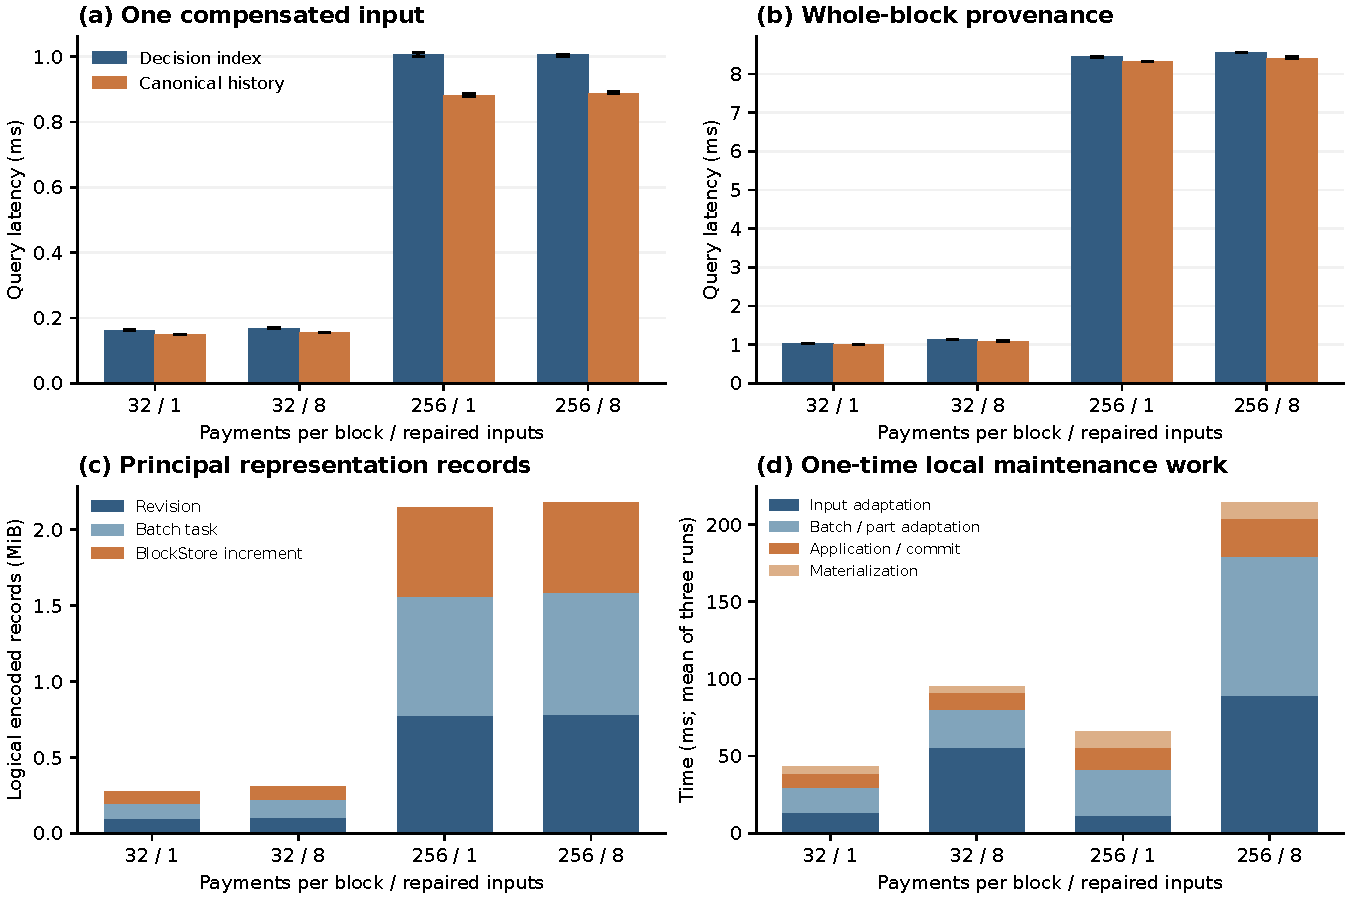
\includegraphics[width=\textwidth]{reader-cost.pdf}
  \caption{读取方的权衡。(a,b) 三个运行级 P50 的中位数及
    最小值--最大值范围。(c) 主要逻辑记录的平均字节数。
    (d) 顺序执行各阶段的平均成本，而不是
    正文历史读取表中的总工作量中位数。}
  \label{fig:reader-cost}
\end{figure*}

\subsection{注入时延配置与逐轮运行结果}
\begin{table}[t]
  \caption{注入时延研究的逐轮运行结果（\texttt{9879f64}）。公开完成和成员完成的 P95 以 s 为单位；链耗时为该轮运行中两条 10 跳链的中位数和最大值，以 ms 为单位。}
  \label{tab:supp-faults}
  \centering
  \small
  \setlength{\tabcolsep}{3.5pt}
  \begin{tabular}{@{}lrrrrr@{}}
    \toprule
    运行 & \shortstack{接收\\P50/P95 (ms)} & \shortstack{公开完成\\P95} & \shortstack{成员完成\\P95} & \shortstack{链耗时\\中位数/最大值} & \shortstack{窗口内\\公开完成数} \\
    \midrule
    H-1   & 42.88/87.52 & 1.277  & 1.361  & 577/619  & -- \\
    H-2   & 41.56/83.20 & 1.288  & 1.375  & 599/619  & -- \\
    H-3   & 40.68/78.23 & 1.263  & 1.344  & 515/542  & -- \\
    L-1   & 81.91/118.22 & 1.315 & 1.410  & 946/980  & -- \\
    L-2   & 83.73/123.52 & 1.360 & 1.468  & 1001/1029 & -- \\
    L-3   & 78.05/111.80 & 1.307 & 1.394  & 815/835  & -- \\
    L-M-1 & 77.65/112.85 & 1.281 & 29.002 & 844/846  & 599 \\
    L-M-2 & 78.31/115.68 & 1.327 & 29.026 & 842/869  & 601 \\
    L-M-3 & 77.71/108.46 & 1.304 & 28.473 & 881/908  & 603 \\
    L-C-1 & 78.18/110.94 & 12.627 & 12.744 & 906/965 & 510 \\
    L-C-2 & 77.33/109.32 & 10.018 & 10.042 & 916/992 & 400 \\
    L-C-3 & 77.41/108.44 & 9.516  & 9.618  & 873/901 & 421 \\
    \bottomrule
  \end{tabular}
\end{table}
固定的四验证者配置运行一个组织的四名成员和一个网关。每个 TCP 方向使用一个有界 FIFO，最多容纳 64 个 16 KiB 数据块，并在到达时间加上所配置时延后释放。所有委员会对等节点地址均使用代理；当验证者保留出站连接时，对重复对等连接的抑制可能使监听代理处于空闲状态。钱包--网关通信、公开 HTTP、钱包交付和存储不注入时延。全部十二轮最终运行均使用 16,384 的文件描述符上限。一次预试运行继承了 256 的描述符上限后，重新执行了整个矩阵；这些受工具影响的预试结果单独保留，不参与合并统计。节点在离线数据库审计之前停止。

每轮运行中的两条链，其耗时均从首次发送计至最后一次认证接收。先在该轮内部取两条链的中位数，再对三次重复运行取中位数。故障窗口 QC 样本组中的请求在暂停至少一秒后发起，并在恢复之前完成接收。成员故障样本组中的全部 QC 恰好包含成员 0、1 和 2。离线验证检查委员会故障各轮运行中的全部 91、91 和 95 个已提交 BlockID。固定集合的提案者优先级表明，被暂停的验证者在每轮运行中有五次第 0 轮提案机会；对应高度均在第~1~轮提交，且不含该验证者的签名。窗口判定使用最晚的有效预提交时间戳，而不是前一高度的区块头时间。

\subsection{归档混合负载中从计划发送到接收的计时}
对于全部 84,000 笔普通付款，先计算记录的接收时间戳减去计划时间戳，再求分位数。沿用归档数据的最近秩计算约定，再取三个运行级 P95 的中位数，得到 N/R/C/P 分别为 304.253、140.007、475.236 和 666.915\,ms。实际发送至接收的 P95 分别为 152.766、139.894、136.491 和 144.205\,ms。前一种口径包含发送前的背压；两种口径都不是将单独的 P95 相加得到的。第 3 轮的部分墙上时钟记录显示发送早于计划时间戳（最小值为 $-13.104$\,ms）；原始差值和计数予以保留，不做截断。这些归档时间戳无法区分定时器唤醒误差与时钟调整，也不用于宣称亚毫秒级的发送调度精度。

\section{当前构建补证与实现对应}
\label{supp:final-evidence}
生产基线为 \texttt{f856c7b}。六轮连续付款与三轮代表性 P 使用相同节点二进制和 Comet 源码；新增 \texttt{payctl} 跟块检查点在全部连续付款轮次启用。工件 \texttt{final-evidence-\allowbreak 2026-10-04} 保存源码、节点指纹、逐笔记录、审计、分析脚本与回归日志。表格由原始 CSV/JSON 生成。

\begin{table}[htbp]
\centering\small
\caption{六轮连续付款；时间自首笔实际发送起计，单位秒。公共列为第 100 笔的公共观察，闭合列为全部付款的成员观察。}
\label{tab:final-evidence-chain}
\begin{tabular}{lrrrrr}\toprule
轮次 & 到账链 & 公共 & 闭合 & 尝试 & 缺口 \\\midrule
r1-fast & 4.726 & 5.451 & 5.495 & 100 & 2 \\
r1-wait & 64.479 & 65.054 & 65.115 & 140 & 0 \\
r2-fast & 4.700 & 5.480 & 5.535 & 100 & 4 \\
r2-wait & 64.670 & 65.280 & 65.300 & 138 & 0 \\
r3-fast & 4.707 & 5.477 & 5.526 & 100 & 1 \\
r3-wait & 64.387 & 64.983 & 65.030 & 136 & 0 \\
\bottomrule\end{tabular}
\end{table}

\noindent\textbf{阶段口径。}一般阶段每轮 100 个付款，跳间过渡每轮 99 个；分别在轮内计算 P50/P95，再取三轮对应分位数的中位数。同一钱包、高度的观测点按付款展开，不作为独立高度样本。区间采用同机 Unix 纳秒时间戳，整链时长采用单调时钟。验证检查点在成功 VerifyBlock 后、PrepareBlock 入口；后事务回调在 Update 返回后，不代表同步刷盘。负值保留为执行重叠。成功取数耗时是提交至完整取数的一部分；各分位数不能相加，返回时间不标识证据最早可得时刻。

\begin{table}[htbp]
\centering\small
\caption{客户端阶段；表项为三轮轮内分位数的中位数，单位毫秒。}
\label{tab:final-evidence-stages}
\begin{tabular}{lrrrr}\toprule
阶段 & fast P50 & fast P95 & wait P50 & wait P95 \\\midrule
发送至应用提交 & 573.703 & 814.807 & 363.470 & 381.553 \\
提交至完整取数 & 395.096 & 440.920 & 285.884 & 314.509 \\
取数至验证检查点 & 0.114 & 0.399 & 0.084 & 0.236 \\
检查点至后事务回调 & 0.940 & 27.496 & 0.128 & 1.343 \\
回调至驱动观察 & 2.669 & 4.649 & 3.099 & 4.713 \\
成功取数调用（重叠） & 9.228 & 26.355 & 0.557 & 7.593 \\
到账至下一跳发送 & 0.269 & 15.228 & 585.442 & 625.777 \\
观察至下一跳构造 & -905.118 & -630.176 & 0.002 & 0.006 \\
下一跳构造至发送 & 0.265 & 15.224 & 0.237 & 11.539 \\
\bottomrule\end{tabular}
\end{table}


\begin{table}[htbp]
\centering\small
\caption{P 的驱动回压；上限命中次数为驱动事件计数，不是拒绝付款数。全部付款闭合。}
\label{tab:final-evidence-pressure}
\begin{tabular}{lrrrr}\toprule
轮次 & 未完成峰值 & 总上限命中 & 快速上限命中 & 计划至到账 P95 (ms) \\\midrule
r1-P & 256 & 7 & 0 & 189.591 \\
r2-P & 256 & 29 & 0 & 326.828 \\
r3-P & 256 & 143 & 917 & 851.742 \\
\bottomrule\end{tabular}
\end{table}

\clearpage
\begingroup
\small
\setlength{\tabcolsep}{3pt}
\setlength{\LTleft}{0pt}
\setlength{\LTright}{0pt}
\setlength{\LTcapwidth}{\textwidth}
\renewcommand{\arraystretch}{1.10}

\begin{longtable}{@{}
    >{\raggedright\arraybackslash}p{0.22\textwidth}
    >{\raggedright\arraybackslash}p{\dimexpr0.48\textwidth-2\tabcolsep\relax}
    >{\raggedright\arraybackslash}p{\dimexpr0.30\textwidth-2\tabcolsep\relax}
    @{}}
\caption{生产基线 \texttt{f856c7b} 的主要证明--实现对应。
共享生产守卫的命题合并列出。完整路径、调用边界和测试断言
保留在工件索引中；本表不代替逐入口清单。}
\label{tab:proof-implementation}\\
\toprule
命题（正文英文名称） &
生产入口与证明相关职责 &
代表性回归证据 \\
\midrule
\endfirsthead

\multicolumn{3}{@{}l}{表~\thetable\ （续）}\\
\toprule
命题（正文英文名称） &
生产入口与证明相关职责 &
代表性回归证据 \\
\midrule
\endhead

\midrule
\multicolumn{3}{r@{}}{续下页}\\
\endfoot

\bottomrule
\endlastfoot

Original-execution agreement
&
Comet overlay 与 \texttt{matchesBlockID} 比较区块哈希和
part-set header。原始分片校验及候选状态转移保持正文与分片配对；
共识、同步和重放保留原始正文及其高度、时间等执行上下文。
&
稳定哈希下的完整身份检查、重标开口及未认证修订拒绝、
保留原始材料的重放测试。Comet 专项证据保留各自记录的构建版本。
\\
\addlinespace[3pt]

Authenticated, unique consumption;
public authorization
&
\texttt{ApproveDirectBytes} 在签名前原子提交锁、Intent、
批准和 debits。
\texttt{CheckTx}、\texttt{ProcessProposal} 和
\texttt{FinalizeBlock} 进入
\texttt{Engine.Check} 及提交验证。
\texttt{Check}/\texttt{ExecuteAt} 固定分派 wire4 的
\texttt{ReserveIncrease}、\texttt{ClockTick}、
\texttt{RepairInput}、\texttt{RepairBatch}、
\texttt{CompensationDecision} 和 \texttt{DirectSubmission}；
\texttt{Execute} 在 direct 模式拒绝 legacy。
完整原始字节缓存不替代
\texttt{EvaluateDirectPaymentAt} 的当前账本检查。
&
\texttt{TestPublicAuthorization\allowbreak AtABCIEntry}；
\texttt{TestDirectModeRejects\allowbreak AlternatePayment\allowbreak Envelopes}；
不同签名成员、相同字节缓存、当前账本重检、
批准持久化及重放测试。
\\
\addlinespace[3pt]

Superseded partial approval;
Residual capacity
&
经认证且成功、Applied 的结果进入
\texttt{reclaimPartial} 和 \texttt{finishLocal}。
正常 CAL 恢复要求已观察到来源成功执行；
局部失效另须满足同配置下共享输入冲突的守卫。
两者均只恢复原始 debits 的剩余部分，
累计进度与跟随游标原子提交。
失效不适用于输入不相交的 Intent 输家。
&
部分批准冲突、多输入重复处理、失败结果不释放、
矛盾原子拒绝、迟到效果拒绝、原始 debit 定位，
以及累计恢复跨重启测试。
\\
\addlinespace[3pt]

Resubmission preserves authorization;
Certificates bound liability, not execution
&
\texttt{recoverExposedSources} 将保留的批准材料与公开 QC
重建并重新验证后入队，不创建批准或 debit。
\texttt{EvaluateDirectPaymentAt} 保留成功交易建立的
全局 Intent 绑定，不因补交而解除冲突。
&
跨组织、多层来源重建与重复暴露；
Subject 隔离；
两轮 Intent 冲突赔付及完整账目检查。
\\
\addlinespace[3pt]

Potential liabilities are funded
&
\texttt{PrepareDirectVector}、提交验证和成员批准绑定
issuer、配置、grant 及 Worker 可用额度。
\texttt{Engine.NewEngine} 按 \texttt{AccountKey}
累计所有 CAL/FUEL grants，并检查各账户授权总额不超过余额。
受保护 CAL 集合覆盖全部组织账户及 CAL grant 账户。
\texttt{GrantShare}、
\texttt{EvaluateReserveIncrease} 和
\texttt{ApplyReserveIncrease} 使用外部非受保护资金及
累计份额差额，不清除已有 debits。
&
无 QC 容量碎片化、补资后完成、补资不解除 2/2 输入分裂、
受保护来源拒绝、共享外部资金及累计取整测试。
隐藏证书集合仍由数学论证覆盖。
\\
\addlinespace[3pt]

Compensation takes effect at most once;
Source repayment
&
\texttt{ExecuteDecision} 对已记录的相同决定返回无新效果，
对不同决定拒绝；无记录时检查 Open、公开到期及原坐标。
\texttt{targetSlot} 仅接受与原 \texttt{OutputID}、
金额及消费者固定字段相符的 \texttt{OriginalFunding}。
赔付与决定记录原子提交。
\texttt{recoverOutput} 在成功来源执行内偿还原 issuer，
使累计回款不超过赔付，且不创建第二份用户输出。
&
重复及冲突决定、迟到来源回款、部分输出赔付、
四跳到达顺序及分叉--合并顺序测试。
\\
\addlinespace[3pt]

CAL conservation;
CAL delay neutrality
&
付款、赔付、回款及补资通过 Overlay 和公共提交生效；
失败转换不写入业务状态。
终态 CAL 比较保留定理的初始状态、
无冲突且来源闭合的付款集合，以及各付款和补资均成功一次的条件，
不比较 FUEL。
&
多种交错与重放下的金额投影；
当前构建 600 笔连续付款和 21,048 笔代表性 P 付款的
逐副本金额审计。
\\
\addlinespace[3pt]

Decision-gated representation authority;
Representation is economically inert
&
\texttt{RepairInput} 和 \texttt{RepairBatch}
均受成功决定及目标槽守卫约束。
\texttt{InputTarget} 及批路径的
\texttt{batchBody}/\texttt{ExecuteBatch}
派生目标替换，保持非目标字节，
检查开口、版本摘要和原完整 BlockID。
写集仅涉及表示状态。
\texttt{EvaluateDirectPaymentAt} 不读取历史
\texttt{Canonical}；
决定已有记录时先作幂等或冲突处理，
否则其他已修订槽不改变其未决定目标槽及固定字段。
这些读侧职责支撑相同高度、时间下后续经济结果不变；
\texttt{DecodePublicExecution} 不产生表示引起的本金效果。
&
双输入原子批次、跨分片批次、适配前赔付，
以及付款--表示金额重放测试。
\\
\addlinespace[3pt]

Identity preservation and installation independence;
local reader contract
&
\texttt{Canonical} 在已执行前缀 $V_H$ 中选择逻辑修订；
\texttt{PrepareMaterialization} 提供精确 Task 材料。
物理版本守卫禁止回滚，重放使用保留的原始材料。
原提交证据验证完整身份相容，不单独授权修订正文。
&
修订顺序、交错队列、原始历史重放、读取等价，
以及真实回款前后 $H=4,5$ 的
\texttt{same\_consumer\_views}：
经济答案一致，原始与授权正文匹配原完整身份，
未适配分片的修改正文被拒绝。
\\
\addlinespace[3pt]

Protected continuation;
Economic closure does not wait for adaptation
&
\texttt{wallet.ReceiveDirect} 检查注册配置、network、
\texttt{Recipient.Owner} 并调用 \texttt{c.VerifyOutput}；
在 \texttt{Update} 内写入 \texttt{DirectCoin}，
拒绝同一 \texttt{OutputID} 对应不一致正文。
\texttt{member.\allowbreak InstallDirectClassified} 先调用
\texttt{VerifyDirectPayment}，再于事务内拒绝
\texttt{Invalidated}，对 \texttt{Observed} 返回无新效果，
检查并保存全部输入及费用输入的 \texttt{Consumed}、
完整 install 材料和 outbox，不新增 reserve。
\texttt{finality.VerifyBlock}、
\texttt{PrepareBlock} 与 \texttt{blockfollow.Commit}
连接认证结果和原子跟随；
\texttt{FreshRecv} 仍是历史前提，不由收款检查单独推出。
经济闭合经 \texttt{ExecuteDecision} 完成，不访问适配服务。
&
批准持久化与后台 INSTALL；
六轮连续链的 297 个提前后继；
P 的 96 次副本--目标检查：
均在表示尚未提交、物化时确认回款完成。
\\

\end{longtable}
\endgroup

\noindent\textbf{前提与证据层级。}
证明覆盖所述模型下的有限轨迹，生产守卫标明实现职责，
回归测试检查具体接受与拒绝轨迹。
四成员组织和四委员、三票法定人数、每组至多一个静态 Byzantine、
一致配置及诚实签名状态不回滚，仍是模型或部署前提；
创世合计备付和受保护 CAL 账户限制另与
\texttt{Engine.NewEngine}、固定命令分派及账户守卫对应。
签名不可伪造、原始承诺绑定及可信 dealer 正确生成并分发
门限 RSA 参数，不由功能测试证明；
固定目标集合的正文与开口收敛还要求唯一有效开口。
历史读取信任一个已验证、已执行且保留相关历史的前缀 $V_H$；
进展仍依赖可用容量、资源及公平传送和包含。
新 \texttt{TestPublicAuthorization\allowbreak AtABCIEntry}
将编码后再篡改授权字段的字节直接送入三个 ABCI 接口，
检查拒绝、\texttt{pendingChanges} 为空及业务库不变。
发送端编码拒绝与接收端拒绝分开记录；
接收端的解码、绑定检查和签名验证属于不同层级，
本测试不确定各用例到达的最深拒绝阶段，
不将编解码拒绝写成已经执行验签。
既有缓存回归区分相同字节复用与当前账本重检。
当前八包回归通过，客户端和测试增量与生产基线分别记录指纹。
Comet 接口、持久重启、网络证据及门限测试保留原有版本和范围，
不被改称为本轮远程下载实验、任意 Byzantine 调度穷举
或机械化证明。

% BEGIN FINAL REVIEW ADDITIONS
\subsection{批准与执行条件}
\begingroup\small
\renewcommand{\arraystretch}{1.15}
\begin{longtable}{@{}>{\raggedright\arraybackslash}p{0.15\textwidth}>{\raggedright\arraybackslash}p{0.25\textwidth}>{\raggedright\arraybackslash}p{0.25\textwidth}>{\raggedright\arraybackslash}p{0.25\textwidth}@{}}
\caption{成员批准与公开执行的对照。D：只取决于提交字节与静态配置的确定性函数；S：对两个不同状态的检查；
L：传送与调度假设。定理~3 仅比较每笔支付与增资都成功的历史；本表不主张带 QC 的支付一定执行。}
\label{tab:sup-checks}\\
\hline
检查项 & 成员批准（\texttt{Approve\allowbreak DirectBytes}） & 公开执行（\texttt{VerifyDirect\allowbreak Submission}、\texttt{EvaluateDirect\allowbreak PaymentAt}） & 关系与主张 \\
\hline
\multicolumn{4}{@{}l}{\textit{D. 确定性检查}} \\
D1 编码、所有者授权、初始资金开口、规则标识、网络/配置/纪元
 & \texttt{PrepareDirect\allowbreak Vector}；身份等于本组织
 & 同一 \texttt{PrepareDirect\allowbreak Vector}，另验当前付款的完整 QC；按配置查组织
 & 固定内容检查共享。成员在本地提交后签单票；公开执行另验证已组成的 QC。 \\
D2 准入向量与额度（CAL 额度含找零；托管下限含每个证书输入一次赔付费用）
 & \texttt{PrepareDirect\allowbreak Vector}
 & \texttt{PrepareDirect\allowbreak Vector}
 & 两侧额度相同。 \\
D3 直接输入证书；价值守恒
 & 核对发行组织配置、规则与输出；每个认证输入恰有一个证书与索引条目；拒绝重复 OutputID 和多余条目；$\sum$输入 $=\sum$输出
 & 同样的绑定检查；评估时 $\sum$输入 $=\sum$输出
 & 等价检查；成员处于已验证的单网络配置内。 \\
\hline
\multicolumn{4}{@{}l}{\textit{S. 状态检查}} \\
S1 输入实例
 & 检查候选/已消费锁；最终本金与用户费用输入使用认证创建记录，认证输入使用匹配证书。输入锁在签名前写入
 & 已消费标记；最终创建记录，或对缺失输出的直接证书
 & 法定人数交叠：不存在两个冲突 QC；QC 排除不同事实对其输入的公开消费。落后可导致拒绝，也可使未签署已执行付款的成员给出局部冲突批准；交叠仍阻止冲突 QC。 \\
S2 Intent
 & 组织本地 Intent $\to$ TxID
 & 全局 Intent $\to$ TxID，成功执行时写入
 & 状态相互独立；可在两方都有效 QC 时冲突（全局 Intent 反例）。 \\
S3 授权、额度、费用
 & 各资源的 Worker 切片 \texttt{Available} $\ge$ 额度；费用输入与授权按成员状态检查
 & CAL：登记不超授权（\texttt{Reserved}+\texttt{Spent} $\le B_g$）；非 CAL：\texttt{updateUsage}；FUEL 账户或费用输入 UTXO
 & CAL 覆盖排除首次登记时授权额度不足，以及对 Open 义务赔付时备付本金不足。其他资源和费用检查仍为独立执行条件。 \\
\hline
\multicolumn{4}{@{}l}{\textit{L. 活性}} \\
L1 纳入、传送、补交
 & 原签署者保留批准并跟随区块链
 & 诚实纳入与公平传送；来源无全局 Intent 冲突
 & 无完成时限，不以超时解锁；闭合不需要适配。 \\
\hline
\end{longtable}
\endgroup


\subsection{恢复与边界证据}
\paragraph{来源自动补交（R）。}
在冻结构建上，一轮计划 2,000 笔普通付款（100/s，20\,s）与三个跨组织父子对，共 2,006 笔，
自动补交开启、适配不暂停。每个父子对中，驱动通过一个既不持久化、不 INSTALL、也不提交的收集器取得父交易三个签名，
驱动自身从不提交父交易；客户端保持在线并继续观察，因此这是扣留发送，不是进程崩溃注入。子交易花费父交易的 TXCer；
子交易公开执行并暴露该证书后，父交易的原签署成员重建并提交父交易。三个义务均以 Fulfilled 结束，无一赔付；
2,006 笔全部闭合，委员会状态哈希一致，outbox 清空，成员 CAL、执行与字节额度预留归零。三个父子对是三个恢复目标，
不是重复实验。时间为客户端观察值；未记录 outbox 的内部创建时间。

\begin{table}[htbp]
\caption{R 中各父子对的观察值（ms）。到账时间自各笔付款自身首次发送起算；
后两列自子交易首次发送起算，为客户端观察点，不是内部恢复时间。}
\label{tab:sup-r}
\centering\small
\begin{tabular}{@{}rrrrr@{}}
\hline
父子对 & 父到账 & 子到账 & 子公开 & 来源 Fulfilled \\
\hline
0 & 100.146 & 116.559 & 1391.849 & 2767.211 \\
1 &  82.988 &  61.749 & 1806.036 & 2958.003 \\
2 &  75.033 & 135.119 & 1286.147 & 2442.890 \\
\hline
\end{tabular}
\end{table}

\paragraph{轮换签署者边界。}
一个确定性回归使用生产批准、公开执行与赔付入口。一个拜占庭成员绕过自身本地额度签名；三个诚实成员按
$(0,1)$、$(0,2)$、$(1,2)$ 轮换共同签署。每轮认证一个 100 CAL、在全局 Intent 上落败的来源，
再由合法子交易消费其输出并扣减发行方备付。取 $B_g=300$，备付依次 $300\to200\to100\to0$，诚实成员累计预留为
$(100,100,0)$、$(200,100,100)$、$(200,200,200)$，第四笔请求被三个诚实成员全部拒绝。重复决定无任何变化，
CAL/FUEL 守恒。该运行达到 $Q_g=B_g$，故表~\ref{tab:s3-ledger} 中两轮即止只对固定签署者集合成立。
它既不度量攻击者收益，也不度量成本：来源输入仍被锁定，FUEL 已花费。

\paragraph{版本桥接。}
721800c 至 9879f64 之间，五个成员生产文件有变动（\texttt{blocks.go}、\texttt{direct.go}、\texttt{outcome.go}、
\texttt{partial\_reclaim.go}、\texttt{source\_recovery.go}）；因此 721800c 的 N/R/C/P 与资本结果保留其原构建，不被继承。
9879f64 至 f856c7b 之间，所检查的成员、委员会、规则、表示、传输、钱包、协议、终局、节点入口、依赖及 Comet 生产文件无变化，
仅客户端与测试文件不同。三个表示核心文件及所列 Comet overlay 文件在三个构建中的 SHA-256 完全相同。旧数字均不改标。

\paragraph{等待模式的重试。}
等待模式 300 笔付款共 414 次尝试（每轮 140、138、136）。客户端在每次失败尝试后固定休眠 50\,ms，
不论原因是传输、HTTP 状态还是读取错误；原日志没有逐次分类。因此 114 次额外尝试在三轮中含 5.7\,s 的固定休眠，
另有未测量的服务时间。我们报告含重试的 $13.70\times$，不推导无重试数字。

\paragraph{清单范围。}
309 项证据清单由 305 项构建源码、\texttt{go.mod}、\texttt{go.sum} 与两个实验驱动组成。
连续链、P 与 R 的节点二进制、客户端及展开后的 Comet 源码完全一致。
\texttt{member} 入口是一个 shell 包装，以 \texttt{GOMAXPROCS=16} 和 \texttt{GOGC=200}
执行 \texttt{member-real}。

\paragraph{发送名额口径。}
驱动先获取快速名额，再等待串行限速发送，到凭证到账后释放。P 第三轮中，全部名额占用时间的
63.31\% 发生在 HTTP 发送之前；该阶段 P95 为 589.422\,ms，记录的限速等待为 589.418\,ms。
在 917 次快速上限检查点，由时间戳重建的已取名额但尚未发送任务中位数为 59，已发送且等待到账的中位数为 5。
重建采用紧邻释放之前的到账时间戳。因此上限命中不能被解释为成员请求缓慢。
总未完成任务的回压仍保留在结果中；本轮未采集运行时跟踪，不把其底层服务延迟归因于 CPU 调度、存储或跟块中的某一项。


\section{补充实验方法}
\label{sec:supp-methods}

\noindent\textbf{构建谱系与部署。}
当前的来源回款代码提交为 \texttt{d99ec92}。归档记录了每个二进制文件的 SHA-256 指纹以及每次运行的配置。当前的九服务续花、回款、存储和短时吞吐系列使用这一来源回款规则。最初的十四服务配对运行使用相同的单义务回款规则，那时批结果标签尚未与直接结果标签分离；当前的跨类型编解码回归覆盖了这一分离。当前存储、内存续花和短时吞吐对照中的成员以 GOGC=200 和 GOMAXPROCS=16 运行；该覆盖设置不应用于委员会、网关或钱包进程。

归档系列保留各自的指纹：运行区间记录基线 \texttt{e3870e1} 与实现 \texttt{a083ff6}；原始续花记录 \texttt{f0c0a274}；资本记录基线 \texttt{8e1fb40} 与实现 \texttt{5807546}；组织路径记录基线 \texttt{bb65af69} 与已验证源码 \texttt{13be856}。归档的批集成使用 \texttt{f82f8cd}；结构性修复计数已在当前代码上重复。来源故障检查点 \texttt{c1ebf2d} 使用已被取代的迟到来源规则，不支持当前的回款论断。

Mac 试验共用一台 M4 Max 主机，16 个 CPU 核和 64\,GiB 内存；结构性微基准运行在 Windows amd64 上。当前的内存链和短时吞吐试验使用内存的服务状态和 NoSync 钱包。回款试验使用磁盘支持的委员会应用状态和 BlockStore，成员与网关在内存中。存储对照仅把成员提交在 bbolt NoSync 与同步事务之间切换。每次运行都从全新创世开始。

另有六次十四服务、磁盘支持的链运行，使用相同的来源回款规则和用户支付的 FUEL。其中三次快速的 100 跳运行耗时 668.960--688.080\,ms；跨跳确认的运行耗时 114.496--118.742\,s。它们属于与正文中九服务结果不同的存储/部署配置。

\noindent\textbf{计时与聚合。}
已认证收款的延迟通常从钱包实际发出第一个 HTTP 请求开始，到收款方验证并在本地原子记录之后结束。资金与来源故障驱动包含少量发送前的构造；它们的比较仅限于同一驱动家族之内。本地 NoSync 事务的完成并不是同步的持久性回执。公共完成与成员完成的时间戳记录的是对已认证执行的观察，而不是委员会的内部提交。发送方的单一单调时钟测量跨站点 ACK 延迟，包含返回路径。收款方可以在前一个发送方收到该 ACK 之前启动其后继付款。提供目标、实际发送速率和含排空的完成速率分别保留。图注区分交易分位数与跨运行的统计量。单次运行内的样本变异性不是对跨运行不确定性的估计。

\noindent\textbf{外部出资的授权控制器。}
资本实验每 200\,ms 采样一次成员可用量。令 $\rho$ 为所声明的每秒 CAL 授权需求，计入每个工作单元中的父请求与子请求；令 $u$ 为认证尚未完成的唯一请求数。控制器设定
\begin{align*}
 b &= 200+100u,\\
 H_{\mathrm{low}} &= \rho\,(0.8\,\mathrm{s})+b,\\
 H_{\mathrm{target}} &= 1.25H_{\mathrm{low}}.
\end{align*}
这里的水位线与突发余量以 CAL 计。当所观察到的最小成员可用量 $A_{\min}$ 低于 $H_{\mathrm{low}}$ 时，所提出的授权额度增量为
\[
 \Delta B=100\left\lceil
 \frac{1.5(H_{\mathrm{target}}-A_{\min})}{100}
 \right\rceil,
\]
并受所配置的授权上限和可用外部资金的约束。同一时刻至多有一次增量在途。其公共命令从外部来源扣款，并原子地向备付金与授权额度入账；其后成员加上由此产生的份额之差，而不清除已有的批准。实验预先提供 $\rho$，而不是估计未知的生产需求。控制器的决定是对实际出资转账的请求，而不是创造备付资本的机制。

\noindent\textbf{资本负载核算。}
每个条件有一次 300-s 的运行，每名成员一个 Worker，并有充足的用户 FUEL。从 3,600 CAL 开始，恒定、速率阶跃和父交易延迟三个条件在外部转账 10,800、18,000 和 19,700 CAL 之后，分别结束于 14,400、21,600 和 23,300 CAL。每个条件完成 6,000 个两跳单元，即 12,000 笔付款，花费 1,128,000 用户 FUEL。相应的固定高备付金对照均能完成；固定低备付金的条件关闭了 6,000 个单元中的 46 个，留下 5,826 个未启动，并记录了 64 笔部分批准的付款。这些类别的单位不同，不能相加为一个付款总数。逐次运行表保留了完整的七个条件的比较，但并不意味着每个条件有三次重复。

\noindent\textbf{身份、资源使用与保留的历史。}
多身份配置使用共享客户端；2,048 个钱包身份并不代表 2,048 个独立的操作系统进程。比较独立输入与十跳付款，三次运行的中位数为每笔付款 12.67 与 15.24 核毫秒，以及每笔付款 59.32 与 71.83\,KiB 的 HTTP 载荷。内存报告把节点总 RSS 与保留的历史，和活动的义务、待处理工作与发件箱分开。因此，历史占用的增加不被报告为付款积压的增加。逐次运行的资源汇总及其归档来源位置包含在归档索引中。

\noindent\textbf{针对特定端点的 Lightning 参考。}
归档的部署使用 LND v0.21.3-beta 和 regtest 中的 Bitcoin Core 31.1，采用同步的 LND 持久化及其 50-ms 通道提交设置。三次全新部署中的每一次都有两个节点和一条直接通道。在 20 次预热转账之后，每次运行使用预先准备的发票，串行地交替发出 100 笔 10,000 聪的付款，以接收方 \texttt{SETTLED} 作为完成事件；报告的 P50/P95 为 282.12/320.17\,ms。另一次 Next 运行以每秒 100 笔的速率发送 300 笔付款，持续 3\,s，使用内存的服务状态和 NoSync 钱包存储。收款方已认证收款的 P50/P95 为 0.9625/1.2075\,ms。负载并发度、持久性和完成语义各不相同，因此这些记录是部署参考，而不是归一化的加速比。


\begin{table}[t]
  \caption{追加式赔付记录与经授权的表示更新（C3）。两者通过相同的经济转移关闭账务；差别在于所存储的历史表示。}
  \label{tab:c3-compare}
  \centering
  \small
  \begin{tabular}{@{}p{0.2\columnwidth}p{0.37\columnwidth}p{0.37\columnwidth}@{}}
    \toprule
    & 追加式记录 & 表示更新（C3） \\
    \midrule
    经济关闭
      & 公共命令中的备付金扣款与义务状态；后继付款不变。
      & 相同的转移与原子步骤，并与一个修订任务一起提交。 \\
    历史表示与原始承诺
      & 原始正文不变；被消费输出的资金来源通过赔付记录的索引找到。
      & 存储的正文指明备付金扣款；交易身份、所有者授权和完整区块身份 $(H_b,P_b)$ 保持不变并经验证。 \\
    实际读者
      & 命令历史与记录的任何读者。
      & 修复构造、安装和本地检查读取修订后的正文；钱包、同步和重放读取原始命令。 \\
    存储与重放
      & 原始区块加记录；重放运行原始命令与赔付事件。
      & 原始区块加修订后的正文、修订和任务；重放运行原始命令与修复事件；同块修复共享分片适配，安装推进到最新的已提交修订。 \\
    进展依赖
      & 赔付记录的公共执行。
      & 赔付与其经验证的修订一起提交，并需要三份适配贡献。 \\
    状态
      & 设计基线；未作为一种模式实现，也未测量。
      & 已实现；成本见正文。 \\
    \bottomrule
  \end{tabular}
\end{table}


\subsection{归档的运行区间系列}
归档的运行区间系列与续花结果相互补充。一个活动组织使用赞助的费用、复用的地址和独立的最终输入。五次各 150,000 笔付款的运行全部完成（图~\ref{fig:operating}）。在目标为每秒 2,000 笔时，两次运行达到含排空的完成速率 1,948.66--1,950.45 笔/秒，收款 P50 为 2.521--2.566\,ms。把目标提高到 2,200，完成速率为 2,103.63--2,106.29 笔/秒。在 2,400 时，达到的速率为 2,174.68，P50/P95 升至 7.174/89.38\,ms，且 4,096 项的待决准入上限记录了 1,635 次命中。运行曲线把达到的完成速率与相应的队列压力配成对。

\begin{figure}[!t]
  \centering
  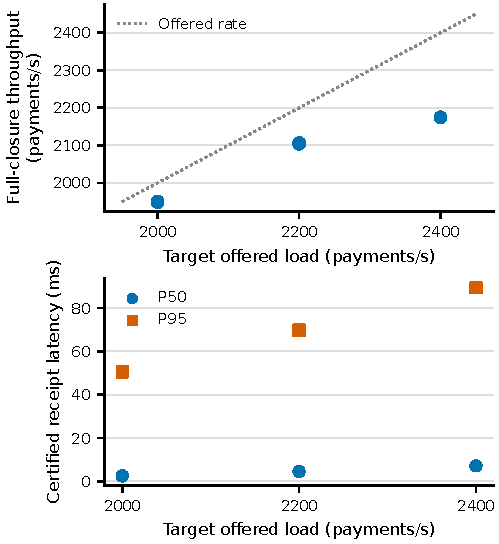
\includegraphics[width=0.62\columnwidth]{operating-point.pdf}
  \caption{运行点随目标提供负载的变化。上：含排空的完成吞吐（笔/秒）。下：收款延迟（ms）。每个点为一次 150,000 笔付款的运行：目标 2,000 两次，2,200 两次，2,400 一次。P50/P95 汇总每次运行内的交易，而不是跨运行的不确定性。所有服务共用一台主机。}
  \label{fig:operating}
\end{figure}

\section{旧构建的实验结果}
\label{sec:archive-results}
以下结果保留原构建、存储与测量条件，属于旧版本证据；当前正文采用冻结评估构建 721800c 的三组实验。旧版性能与 CPU 测量来自不同构建和负载，不能混用为同一系统的容量推导。

\subsection{无需逐跳结算的连续花费}
\label{archive:sec:eval-continuation}

我们把认证续花与在各跳之间等待公共执行进行比较。在基线版本上，100 跳链到达最后一次认证接收的中位耗时为 158.846\,ms，而每一跳都等待公共确认时为 65.204\,s。三个钱包轮流转账 100 CAL，每笔支付都由其前一笔的输出在线构造，并用自己的最终 FUEL 支付费用。每种模式重复三次，在九服务的内存配置上共得到六次运行、600 笔支付。两种模式都以最后一次认证接收为终点，等待模式则在各跳\emph{之间}增加一次公共确认。在委员会 commit、flush 和 gossip 设置分别为 250、10 和 10\,ms 时，公共执行及其观察每跳耗时约 0.65\,s。认证续花消除了收款方路径上的这段等待。

图~\ref{archive:fig:continuation} 给出六次整链耗时。快速运行耗时 158.492--159.905\,ms。快速模式下全部 297 个后继请求，都消费其前一笔已认证的输出，并在该输出的认证接收之后、其公共完成被观察到之前发出。一个单输入、单输出的 TXCer 为 779 字节，请求在第一跳为 1,979 字节，之后为 2,766 字节。对于这种交易形态，直接证据的大小在全部 100 跳中保持不变，因为每个请求携带的是其直接输入的证书，而不是祖先链。

\begin{figure}[t]
  \centering
  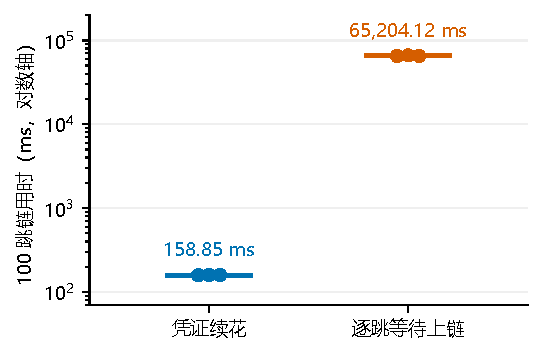
\includegraphics[width=\columnwidth]{continuation-current-zh.pdf}
  \caption{基线版本上 100 跳链到最后一次认证接收的耗时。圆点为每种模式的三次独立运行；横线标出它们的中位数。对数时间轴在两种模式中包含相同的终点。只有等待式基线要求在相邻支付之间进行公共确认。}
  \label{archive:fig:continuation}
\end{figure}

为检验这一优势是否依赖于内存中的成员存储，我们在九服务的落盘配置上，使用 NoSync 钱包和用户自付 FUEL，做了三组配对的 100 跳试验。这些试验仅在成员存储上不同（NoSync 或同步；顺序为 N/S、S/N、N/S），每组之后各跟一条同步的等待链。中位耗时分别是：NoSync 续花 681.127\,ms，同步续花 4.471\,s，同步等待 65.013\,s。因此在成员提交为同步时，认证续花仍比等待快 14.5 倍。全部 900 笔支付完成，且各委员会状态一致。

在归档的交付门控版本上，认证之后有一个投递门控，它等待三名成员 INSTALL 完整材料，或等待经认证的公共执行成功。该门控不收集第二个签名法定人数；改为立即交付会缩短续花。在每秒 200 笔支付、持续 30\,s 的条件下，每种模式三次配对运行各完成 6,000 笔支付，运行级接收 P50 的中位数从有门控时的 2.167\,ms 降到 1.300\,ms（下降 40.0\%）。另外的 100 跳试验从 287.983 降到 200.356\,ms（下降 30.43\%）。授权不变，补充材料列出了配对运行。

\subsection{有资金支撑的关闭与偿还}
\label{archive:sec:eval-liabilities}

本实验检验赔付是否保持后继支付不变，以及每次赔付是否在其源交易随后执行时恰好偿还一次。

\noindent\textbf{赔付与偿还矩阵（基线版本）。}
九次运行使用随机种子 23、37 和 59，被扣留父交易的比例分别为 0\%、1\% 和 5\%。每次运行按每秒 20 个两跳单元的速率提供负载，持续 60\,s（1,200 个单元，2,400 笔支付），对应一份固定的 60,000-CAL 备付金，使用用户自付 FUEL 且不充值。九服务部署使用落盘的委员会应用状态和 BlockStore，成员和网关在内存中，钱包为 NoSync。驱动程序只有在每个被扣留父交易的赔付已在全部四个副本上提交并完成安装之后，才释放该父交易，所以每个被扣留的源交易都在 30-s 公共时间期限之后被赔付，并在其后执行。

全部 21,600 笔支付都完成关闭。216 次赔付（1\% 的每次运行 12 次，5\% 的每次运行 60 次）各自之后都有偿还。每次运行结束时，没有义务处于 Open 或 Repaired，缺口为零，净 Spent 和 Reserved 为零，备付金回到 60,000\,CAL（表~\ref{archive:tab:eval-audit}）。所采样到的最低备付金在 1\% 时为 59,800--59,900\,CAL，在 5\% 时为 59,600\,CAL。它反映的是驱动程序的释放节奏，不是备付金规模的结果，补充材料绘出了三次 5\% 运行的轨迹。正常子支付的运行级接收 P50 为 1.185--1.251\,ms。从期限起算，委员会提交（在该版本中它承载历史表示）的观察时间中位数为 1.003--1.254\,s，全部四个副本上完成修订区块体物理安装的时间中位数为 1.257--1.761\,s（P95 最高 2.015\,s）；两者都包含 250-ms 的观察轮询。每笔正常支付花费 94 FUEL，每次赔付增加 5，奖励、销毁与退款之和等于费用上限，Held 为零。

\begin{table}[t]
  \caption{赔付与偿还矩阵的收尾审计。每一列都被三个随机种子复现；每次运行有 2,400 笔支付。备付金数值以 CAL 计，费用数值以千 FUEL 计，费用上限为各笔支付最大值之和。}
  \label{archive:tab:eval-audit}
  \centering
  \small
  \begin{tabular}{@{}lrrr@{}}
    \toprule
    被扣留父交易比例 & 0\% & 1\% & 5\% \\
    \midrule
    赔付 / 偿还次数 & 0 & 12 & 60 \\
    赔付 / 偿还 CAL & 0 & 1,200 & 6,000 \\
    最终备付金 & 60,000 & 60,000 & 60,000 \\
    未关闭 / 净 Spent & 0 & 0 & 0 \\
    费用上限总额 & 2,400 & 2,400 & 2,400 \\
    Rewards & 201.600 & 201.660 & 201.900 \\
    Burned & 24.000 & 24.000 & 24.000 \\
    Refunded & 2,174.400 & 2,174.340 & 2,174.100 \\
    Remaining Held & 0 & 0 & 0 \\
    \bottomrule
  \end{tabular}
\end{table}

账本层面的回归测试直接覆盖到达顺序：四跳链的全部 24 种到达顺序，在有到期赔付与无到期赔付两种情形下，各取三种签发组织序列，共得到 144 条轨迹；另有 48 条拆分--合并轨迹，在两种赔付模式下，改变一个 40/60 拆分、两条分支及其合并的全部到达顺序。192 条轨迹中的每一步都保持独立计算的资产投影守恒。每条轨迹结束时，各签发组织的备付金恢复，Spent 与 Reserved 为零，$\mathsf{Paid}=\mathsf{Rec}$，已消费的输入仍保持已消费。

两个十四服务的对照实验区分永久损失与延迟偿还。父交易始终不到达时，孙支付保留其 100 CAL，而负责的签发组织的备付金仍然低 100 CAL。当跨组织链以孙支付最先到达的顺序到达时，中间源交易关闭其自己的直接义务，根签发组织被赔付的 100 CAL 在根交易其后执行时得到偿还。两种情况下四个委员会状态一致，缺席的父交易自身的费用和工作预留可能保持未清偿。

三组配对的十四服务运行使用基线版本的初始构建（在批处理结果标签分离之前），每次 4,000 笔支付、速率 100 笔/秒，其正常运行与扣留源交易运行最终的所有者持有和备付金余额完全一致，与主文的 CAL 延迟中性定理 一致。并发赔付使接收 P95 升高为 1.98--2.21 倍，这些配对不能区分造成这一升高的具体环节。

一个使用 NoSync 钱包的存储对照把成员提交单独隔离出来：NoSync 成员时接收 P50 为 1.0\,ms，同步提交时为 43--52\,ms。

早期版本的资本系列（每个条件一次运行、没有赔付）表明，10,800--19,700\,CAL 的外部新增，足以维持从 3,600-CAL 起步、各含 6,000 个两跳单元的 300-s 运行，而固定 3,600-CAL 的对照只关闭了 6,000 个单元中的 46 个。

\subsection{跨注册组织的续花}
\label{archive:sec:eval-network}

为测量通信距离的影响，我们在补充材料所记录的一个归档版本上运行了双组织套件：两个钱包进程各持 32 个身份，经 64 个 lane 发送，每个组织提供 50 笔/秒，24 次运行共完成 342,000 笔支付。延迟比较使用十跳的同组织与跨组织负载，注入的 HTTP RTT 为 0、20 和 100\,ms，每个条件重复三次。每个代理方向增加一半的 RTT，组织内部认证和委员会 P2P 不注入延迟。

\begin{figure}[t]
  \centering
  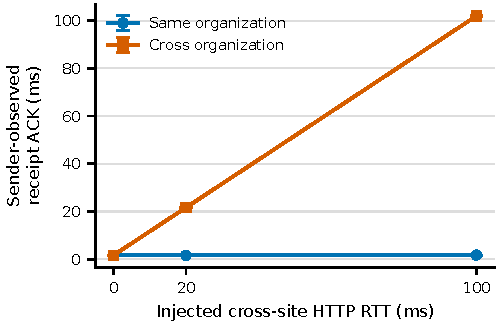
\includegraphics[width=\columnwidth]{network.pdf}
  \caption{ACK 延迟（ms）与注入的跨站点 HTTP RTT（ms）的关系。每个点是前 120-s 样本组的三个运行级 P50 的中位数；误差条跨越这些 P50 的最小值与最大值。总提供速率为 100 笔/秒。委员会 P2P 未加延迟。}
  \label{archive:fig:network}
\end{figure}

对共同的前 120-s 样本组，三个运行级跨组 ACK P50 的中位数依次为 1.632、21.658 和 101.967\,ms，同组数值范围为 1.615--1.744\,ms（图~\ref{archive:fig:network}）。跨组 ACK P50 随注入 RTT 变化，测得的超出部分为 1.6--2.0\,ms。ACK 包含返回路径，但收款方可以在接受之后即刻发起其后继交易，无需等待该 ACK 到达前一个发送方。在 100-ms 跨组 RTT 下，三次 300-s 运行各完成 30,000 笔支付；待处理峰值为 106--110，并能排空，没有持续的尾部增长。该实验在一台物理主机内隔离出 HTTP 路径延迟。

\subsection{运行容量与服务可用性}
\label{archive:sec:eval-operating}

\noindent\textbf{独立输入吞吐（基线版本）。}
三次各 30,000 笔支付的运行以 2,000 笔/秒为目标，使用九服务的内存配置、NoSync 钱包和经授权的组织代付 FUEL。成员进程使用 200\% 的 Go GC 目标和 16 个运行时处理器。全部支付完成，四个委员会状态一致。含排空的完成速率为 1,750.27、1,820.91 和 1,887.31 笔/秒，历时 15.9--17.1\,s，接收 P50 为 2.646、2.842 和 2.824\,ms，P95 为 47.9、49.1 和 48.0\,ms。驱动程序记录到有 6,551--7,570 笔支付需要等待快速接收准入名额，P95 派发滞后为 179--229\,ms，所以提供的负载并不是均匀的 2,000 笔/秒。这些是基线版本上的短时完成测量，没有在 decision-first 版本上重新测量；该版本在普通支付上的开销由上文的六次运行对比检验。补充材料说明了 150,000 笔支付系列所用的版本和时长。

在归档版本上，冗余认证与已 INSTALL 的证据在所述故障下维持服务。九次每秒 200 笔的运行完成 216,000 笔支付，其间有一个成员被延迟或暂停 30\,s。网关丢失对照中，一名成员持有经 INSTALL 复制的完整材料，备用提交在 INSTALL 之后 2.503--2.508\,s 出现。冲突对照既没有出现相互冲突的双 QC，也没有重复的本金或费用效果，而部分批准仍然是一种额度代价。

补充材料第~S2 节的多身份测量报告每笔支付的 CPU 和 HTTP 负载开销；2,048 个身份共享客户端。历史内存增长与积压分别报告。该节还给出 LND regtest 参照，其完成事件、持久化设置和负载并发度与 Next 的测量不同。

\clearpage
\section{逐轮实验记录}
\begin{table}[!ht]
\centering\small
\caption{归档的单组织运行点实验。每轮发送并完成150,000笔付款。
实际发送速率与完成速率的单位为笔付款/s，认证接收分位数的单位为ms。
完成速率计入最终后台排空时间。峰值表示后台处理尚未完成的付款数峰值；
上限触发次数表示4,096笔未完成付款上限的触发次数。}
\label{tab:supp-throughput}
\begin{tabular}{@{}rrrrrrrr@{}}
\toprule
轮次 & 目标 & 实际发送 & 完成 & P50 & P95 & 峰值 & 上限触发次数 \\
\midrule
1 & 2000 & 1,964.53 & 1,948.66 & 2.521 & 50.499 & 2159 & 0 \\
2 & 2000 & 1,969.65 & 1,950.45 & 2.566 & 50.761 & 2205 & 0 \\
3 & 2200 & 2,127.70 & 2,103.63 & 4.538 & 69.463 & 2655 & 0 \\
4 & 2200 & 2,127.15 & 2,106.29 & 4.553 & 69.945 & 2548 & 0 \\
5 & 2400 & 2,206.95 & 2,174.68 & 7.174 & 89.376 & 4096 & 1635 \\
\bottomrule
\end{tabular}
\end{table}
\begin{table}[!ht]
\centering\small
\caption{当前来源回款矩阵的逐轮记录。每轮在 60 秒内提供 1,200 个两跳单元（2,400 笔付款）。收款分位数为正常子付款的毫秒数；总耗时及截止至全部副本物理安装的观察中位数为秒，后者含 250 毫秒轮询。每轮结束时备付余额为 60,000 CAL，净支出及缺口为零。}
\label{tab:supp-liability}
\begin{tabular}{@{}rrrrrrr@{}}
\toprule
种子 & 扣留率 & 赔付/回款 & 总耗时 & 子 P50 & 子 P95 & 安装 P50 \\
\midrule
23 & 0\% & 0/0 & 61.540 & 1.251 & 1.620 & -- \\
23 & 1\% & 12/12 & 90.225 & 1.185 & 1.432 & 1.759 \\
23 & 5\% & 60/60 & 90.096 & 1.191 & 1.536 & 1.257 \\
37 & 0\% & 0/0 & 61.595 & 1.199 & 1.559 & -- \\
37 & 1\% & 12/12 & 91.935 & 1.190 & 1.479 & 1.509 \\
37 & 5\% & 60/60 & 91.530 & 1.192 & 1.426 & 1.257 \\
59 & 0\% & 0/0 & 61.550 & 1.191 & 1.461 & -- \\
59 & 1\% & 12/12 & 90.595 & 1.193 & 1.452 & 1.761 \\
59 & 5\% & 60/60 & 90.346 & 1.194 & 1.494 & 1.507 \\
\bottomrule
\end{tabular}
\end{table}
\begin{table}[!ht]
\centering\small
\caption{归档的有限备付实验。每个条件进行一轮300-s运行，资金数值单位为CAL。
已关闭计数以两跳单位计。自适应增加来自外部资金账户的实际转账。
均值是对300秒输入窗口内采样余额进行积分所得的组织CAL余额时间平均值。}
\label{tab:supp-reserve}
\begin{tabular}{@{}lrrrrr@{}}
\toprule
条件 & 初始 & 新增 & 最终 & 均值 & 已关闭 \\
\midrule
恒定 / 固定低备付 & 3,600 & 0 & 3,600 & 3,600.0 & 46/6000 \\
恒定 / 固定高备付 & 14,400 & 0 & 14,400 & 14,400.0 & 6000/6000 \\
恒定 / 自适应 & 3,600 & 10,800 & 14,400 & 13,801.8 & 6000/6000 \\
阶跃 / 固定高备付 & 21,600 & 0 & 21,600 & 21,600.0 & 6000/6000 \\
阶跃 / 自适应 & 3,600 & 18,000 & 21,600 & 14,078.7 & 6000/6000 \\
延迟 / 固定高备付 & 28,800 & 0 & 28,800 & 28,800.0 & 6000/6000 \\
延迟 / 自适应 & 3,600 & 19,700 & 23,300 & 20,611.2 & 6000/6000 \\
\bottomrule
\end{tabular}
\end{table}


\begin{table}[!ht]
\centering\small
\caption{同步成员续花对照：每轮 100 跳，九服务磁盘配置，用户自付 FUEL，钱包 NoSync。单位为秒，终点为末跳认证收款。N/S 表示两种快速模式的配对顺序，每对之后运行同步等待链。}
\label{tab:supp-sync-chain}
\begin{tabular}{@{}rlrrr@{}}
\toprule
轮对 & 顺序 & NoSync 续花 & 同步续花 & 同步等待 \\
\midrule
1 & N/S & 0.681127 & 4.492812 & 64.969480 \\
2 & S/N & 0.705604 & 4.309984 & 65.193522 \\
3 & N/S & 0.636821 & 4.470844 & 65.012947 \\
\midrule
中位数 & & 0.681127 & 4.470844 & 65.012947 \\
\bottomrule
\end{tabular}
\end{table}

\bibliographystyle{IEEEtran}
\bibliography{references}
\end{document}
